% python classes slides - classes_introduction
% (c) 2012 Kostiantyn Danylov aka koder 
% koder.mail@gmail.com
% distributed under CC-BY licence
% http://creativecommons.org/licenses/by/3.0/deed.en

\documentclass{article}
% XeLaTeX
\usepackage{xltxtra}
\usepackage{xunicode}
\usepackage{listings}
\usepackage[landscape]{geometry}

% Fonts
\setmainfont{DejaVu Sans} %{Arial}
\newfontfamily\cyrillicfont{Nimbus Roman No9 L} %{Arial}
\setmonofont{Courier New}
%\setmonofont{Ubuntu Mono}

%\setmonofont{DejaVu Sans Mono}

% Lang
\usepackage{polyglossia}
\setmainlanguage{russian}
\setotherlanguage{english}
\usepackage[dvipsnames,table]{xcolor}


\ifx\pdfoutput\undefined
\usepackage{graphicx}
\else
\usepackage[pdftex]{graphicx}
\fi

\lstset{
	language=python,
	keywordstyle=\color{Emerald},%\texttt, 
	commentstyle=\color{OliveGreen},%\texttt,
	stringstyle=\color{Bittersweet},%\texttt,
	tabsize=4,
	numbers=left,
	xleftmargin=10pt,
	morekeywords={with,as},	
	numberstyle=\large,
	%identifierstyle=\texttt,
	%basicstyle=\texttt,
}

\usepackage{hyperref}

\hypersetup{
	colorlinks=true,
	urlcolor=blue
}

\usepackage{float}
%\floatstyle{boxed} 
%\restylefloat{figure}
\usepackage[normalem]{ulem}


\makeatletter
\def\PY@reset{\let\PY@it=\relax \let\PY@bf=\relax%
    \let\PY@ul=\relax \let\PY@tc=\relax%
    \let\PY@bc=\relax \let\PY@ff=\relax}
\def\PY@tok#1{\csname PY@tok@#1\endcsname}
\def\PY@toks#1+{\ifx\relax#1\empty\else%
    \PY@tok{#1}\expandafter\PY@toks\fi}
\def\PY@do#1{\PY@bc{\PY@tc{\PY@ul{%
    \PY@it{\PY@bf{\PY@ff{#1}}}}}}}
\def\PY#1#2{\PY@reset\PY@toks#1+\relax+\PY@do{#2}}

\expandafter\def\csname PY@tok@gd\endcsname{\def\PY@tc##1{\textcolor[rgb]{0.63,0.00,0.00}{##1}}}
\expandafter\def\csname PY@tok@gu\endcsname{\let\PY@bf=\textbf\def\PY@tc##1{\textcolor[rgb]{0.50,0.00,0.50}{##1}}}
\expandafter\def\csname PY@tok@gt\endcsname{\def\PY@tc##1{\textcolor[rgb]{0.00,0.25,0.82}{##1}}}
\expandafter\def\csname PY@tok@gs\endcsname{\let\PY@bf=\textbf}
\expandafter\def\csname PY@tok@gr\endcsname{\def\PY@tc##1{\textcolor[rgb]{1.00,0.00,0.00}{##1}}}
\expandafter\def\csname PY@tok@cm\endcsname{\let\PY@it=\textit\def\PY@tc##1{\textcolor[rgb]{0.25,0.50,0.50}{##1}}}
\expandafter\def\csname PY@tok@vg\endcsname{\def\PY@tc##1{\textcolor[rgb]{0.10,0.09,0.49}{##1}}}
\expandafter\def\csname PY@tok@m\endcsname{\def\PY@tc##1{\textcolor[rgb]{0.40,0.40,0.40}{##1}}}
\expandafter\def\csname PY@tok@mh\endcsname{\def\PY@tc##1{\textcolor[rgb]{0.40,0.40,0.40}{##1}}}
\expandafter\def\csname PY@tok@go\endcsname{\def\PY@tc##1{\textcolor[rgb]{0.50,0.50,0.50}{##1}}}
\expandafter\def\csname PY@tok@ge\endcsname{\let\PY@it=\textit}
\expandafter\def\csname PY@tok@vc\endcsname{\def\PY@tc##1{\textcolor[rgb]{0.10,0.09,0.49}{##1}}}
\expandafter\def\csname PY@tok@il\endcsname{\def\PY@tc##1{\textcolor[rgb]{0.40,0.40,0.40}{##1}}}
\expandafter\def\csname PY@tok@cs\endcsname{\let\PY@it=\textit\def\PY@tc##1{\textcolor[rgb]{0.25,0.50,0.50}{##1}}}
\expandafter\def\csname PY@tok@cp\endcsname{\def\PY@tc##1{\textcolor[rgb]{0.74,0.48,0.00}{##1}}}
\expandafter\def\csname PY@tok@gi\endcsname{\def\PY@tc##1{\textcolor[rgb]{0.00,0.63,0.00}{##1}}}
\expandafter\def\csname PY@tok@gh\endcsname{\let\PY@bf=\textbf\def\PY@tc##1{\textcolor[rgb]{0.00,0.00,0.50}{##1}}}
\expandafter\def\csname PY@tok@ni\endcsname{\let\PY@bf=\textbf\def\PY@tc##1{\textcolor[rgb]{0.60,0.60,0.60}{##1}}}
\expandafter\def\csname PY@tok@nl\endcsname{\def\PY@tc##1{\textcolor[rgb]{0.63,0.63,0.00}{##1}}}
\expandafter\def\csname PY@tok@nn\endcsname{\let\PY@bf=\textbf\def\PY@tc##1{\textcolor[rgb]{0.00,0.00,1.00}{##1}}}
\expandafter\def\csname PY@tok@no\endcsname{\def\PY@tc##1{\textcolor[rgb]{0.53,0.00,0.00}{##1}}}
\expandafter\def\csname PY@tok@na\endcsname{\def\PY@tc##1{\textcolor[rgb]{0.49,0.56,0.16}{##1}}}
\expandafter\def\csname PY@tok@nb\endcsname{\def\PY@tc##1{\textcolor[rgb]{0.00,0.50,0.00}{##1}}}
\expandafter\def\csname PY@tok@nc\endcsname{\let\PY@bf=\textbf\def\PY@tc##1{\textcolor[rgb]{0.00,0.00,1.00}{##1}}}
\expandafter\def\csname PY@tok@nd\endcsname{\def\PY@tc##1{\textcolor[rgb]{0.67,0.13,1.00}{##1}}}
\expandafter\def\csname PY@tok@ne\endcsname{\let\PY@bf=\textbf\def\PY@tc##1{\textcolor[rgb]{0.82,0.25,0.23}{##1}}}
\expandafter\def\csname PY@tok@nf\endcsname{\def\PY@tc##1{\textcolor[rgb]{0.00,0.00,1.00}{##1}}}
\expandafter\def\csname PY@tok@si\endcsname{\let\PY@bf=\textbf\def\PY@tc##1{\textcolor[rgb]{0.73,0.40,0.53}{##1}}}
\expandafter\def\csname PY@tok@s2\endcsname{\def\PY@tc##1{\textcolor[rgb]{0.73,0.13,0.13}{##1}}}
\expandafter\def\csname PY@tok@vi\endcsname{\def\PY@tc##1{\textcolor[rgb]{0.10,0.09,0.49}{##1}}}
\expandafter\def\csname PY@tok@nt\endcsname{\let\PY@bf=\textbf\def\PY@tc##1{\textcolor[rgb]{0.00,0.50,0.00}{##1}}}
\expandafter\def\csname PY@tok@nv\endcsname{\def\PY@tc##1{\textcolor[rgb]{0.10,0.09,0.49}{##1}}}
\expandafter\def\csname PY@tok@s1\endcsname{\def\PY@tc##1{\textcolor[rgb]{0.73,0.13,0.13}{##1}}}
\expandafter\def\csname PY@tok@sh\endcsname{\def\PY@tc##1{\textcolor[rgb]{0.73,0.13,0.13}{##1}}}
\expandafter\def\csname PY@tok@sc\endcsname{\def\PY@tc##1{\textcolor[rgb]{0.73,0.13,0.13}{##1}}}
\expandafter\def\csname PY@tok@sx\endcsname{\def\PY@tc##1{\textcolor[rgb]{0.00,0.50,0.00}{##1}}}
\expandafter\def\csname PY@tok@bp\endcsname{\def\PY@tc##1{\textcolor[rgb]{0.00,0.50,0.00}{##1}}}
\expandafter\def\csname PY@tok@c1\endcsname{\let\PY@it=\textit\def\PY@tc##1{\textcolor[rgb]{0.25,0.50,0.50}{##1}}}
\expandafter\def\csname PY@tok@kc\endcsname{\let\PY@bf=\textbf\def\PY@tc##1{\textcolor[rgb]{0.00,0.50,0.00}{##1}}}
\expandafter\def\csname PY@tok@c\endcsname{\let\PY@it=\textit\def\PY@tc##1{\textcolor[rgb]{0.25,0.50,0.50}{##1}}}
\expandafter\def\csname PY@tok@mf\endcsname{\def\PY@tc##1{\textcolor[rgb]{0.40,0.40,0.40}{##1}}}
\expandafter\def\csname PY@tok@err\endcsname{\def\PY@bc##1{\setlength{\fboxsep}{0pt}\fcolorbox[rgb]{1.00,0.00,0.00}{1,1,1}{\strut ##1}}}
\expandafter\def\csname PY@tok@kd\endcsname{\let\PY@bf=\textbf\def\PY@tc##1{\textcolor[rgb]{0.00,0.50,0.00}{##1}}}
\expandafter\def\csname PY@tok@ss\endcsname{\def\PY@tc##1{\textcolor[rgb]{0.10,0.09,0.49}{##1}}}
\expandafter\def\csname PY@tok@sr\endcsname{\def\PY@tc##1{\textcolor[rgb]{0.73,0.40,0.53}{##1}}}
\expandafter\def\csname PY@tok@mo\endcsname{\def\PY@tc##1{\textcolor[rgb]{0.40,0.40,0.40}{##1}}}
\expandafter\def\csname PY@tok@kn\endcsname{\let\PY@bf=\textbf\def\PY@tc##1{\textcolor[rgb]{0.00,0.50,0.00}{##1}}}
\expandafter\def\csname PY@tok@mi\endcsname{\def\PY@tc##1{\textcolor[rgb]{0.40,0.40,0.40}{##1}}}
\expandafter\def\csname PY@tok@gp\endcsname{\let\PY@bf=\textbf\def\PY@tc##1{\textcolor[rgb]{0.00,0.00,0.50}{##1}}}
\expandafter\def\csname PY@tok@o\endcsname{\def\PY@tc##1{\textcolor[rgb]{0.40,0.40,0.40}{##1}}}
\expandafter\def\csname PY@tok@kr\endcsname{\let\PY@bf=\textbf\def\PY@tc##1{\textcolor[rgb]{0.00,0.50,0.00}{##1}}}
\expandafter\def\csname PY@tok@s\endcsname{\def\PY@tc##1{\textcolor[rgb]{0.73,0.13,0.13}{##1}}}
\expandafter\def\csname PY@tok@kp\endcsname{\def\PY@tc##1{\textcolor[rgb]{0.00,0.50,0.00}{##1}}}
\expandafter\def\csname PY@tok@w\endcsname{\def\PY@tc##1{\textcolor[rgb]{0.73,0.73,0.73}{##1}}}
\expandafter\def\csname PY@tok@kt\endcsname{\def\PY@tc##1{\textcolor[rgb]{0.69,0.00,0.25}{##1}}}
\expandafter\def\csname PY@tok@ow\endcsname{\let\PY@bf=\textbf\def\PY@tc##1{\textcolor[rgb]{0.67,0.13,1.00}{##1}}}
\expandafter\def\csname PY@tok@sb\endcsname{\def\PY@tc##1{\textcolor[rgb]{0.73,0.13,0.13}{##1}}}
\expandafter\def\csname PY@tok@k\endcsname{\let\PY@bf=\textbf\def\PY@tc##1{\textcolor[rgb]{0.00,0.50,0.00}{##1}}}
\expandafter\def\csname PY@tok@se\endcsname{\let\PY@bf=\textbf\def\PY@tc##1{\textcolor[rgb]{0.73,0.40,0.13}{##1}}}
\expandafter\def\csname PY@tok@sd\endcsname{\let\PY@it=\textit\def\PY@tc##1{\textcolor[rgb]{0.73,0.13,0.13}{##1}}}

\def\PYZbs{\char`\\}
\def\PYZus{\char`\_}
\def\PYZob{\char`\{}
\def\PYZcb{\char`\}}
\def\PYZca{\char`\^}
\def\PYZam{\char`\&}
\def\PYZlt{\char`\<}
\def\PYZgt{\char`\>}
\def\PYZsh{\char`\#}
\def\PYZpc{\char`\%}
\def\PYZdl{\char`\$}
\def\PYZti{\char`\~}
% for compatibility with earlier versions
\def\PYZat{@}
\def\PYZlb{[}
\def\PYZrb{]}
\makeatother

\begin{document}
\LARGE

%-------------------------------------------------------------------------------
\begin{center} Задача \end{center}
    Написать обработчик выражения, состоящего из -, +, скобок и чисел.
    В первую очередь нас интересует вычислитель.
    (Пусть у нас уже есть парсер выражения).
    \pause

\begin{lstlisting}
    expression = "1 + 2 + ( 4 - 3 )"
    pexpr = parse(expression)
    print pexpr # ('+', ('+', 1, 2), ('-', 3 , 4))
\end{lstlisting}
    \begin{center} 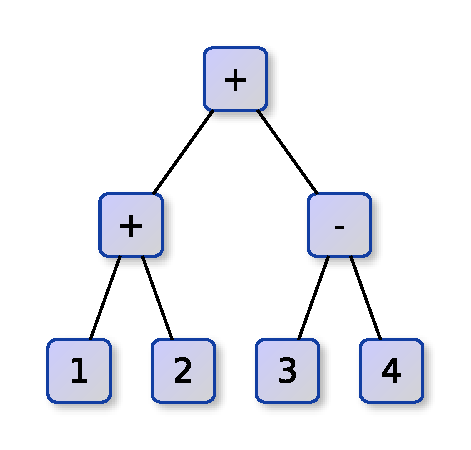
\includegraphics{images/parse_tree.eps} \end{center}     
\newpage

%-------------------------------------------------------------------------------
\begin{center} Решение 1 \end{center}
\begin{lstlisting}
    def evaluate(val):
        if isinstance(val, int):
            res = val
        else:
            operator, oper1, oper2 = val
            assert operator in "+-", "Unknown operator " + operator

            v1 = evaluate(oper1)
            v2 = evaluate(oper2)

            if operator == '+':
                res = v1 + v2
            elif operator == '-':
                res = v1 - v2

        return res
\end{lstlisting}
\newpage

%-------------------------------------------------------------------------------
\begin{center} Задача 2 \end{center}
    Добавить в выражение поддержку * и /
\newpage

%-------------------------------------------------------------------------------
\begin{center} Решение 2 \end{center}
\begin{lstlisting}
    def evaluate(val):
        if isinstance(val, int):
            res = val
        else:
            operator, oper1, oper2 = val
            assert operator in "+-*/", "Unknown operator " + operator

            v1 = evaluate(oper1)
            v2 = evaluate(oper2)

            if operator == '+':
                res = v1 + v2
            elif operator == '-':
                res = v1 - v2
            elif operator == '*':
                res = v1 * v2
            elif operator == '/':
                res = v1 / v2
        return res
\end{lstlisting}
\newpage

%-------------------------------------------------------------------------------
\begin{center} Проблема 1 \end{center}
\begin{itemize}
    \item Добавление новых типов требует изменения функции evaluate
\end{itemize}
\newpage

%-------------------------------------------------------------------------------
\begin{center} Решение 3 \end{center}
    Добавить в выражение поддержку * и /
\begin{lstlisting}
    def evaluate_2(val):
        if isinstance(val, int):
            res = val
        else:
            operator, oper1, oper2 = val
            v1 = evaluate_2(oper1)
            v2 = evaluate_2(oper2)

            if operator == '*':
                res = v1 * v2
            elif operator == '/':
                res = v1 / v2
            else:
                res = evaluate((operator, v1, v2))

        return res
\end{lstlisting}
\newpage

%-------------------------------------------------------------------------------
\begin{center} Проблема 2 \end{center}
\begin{itemize}
    \item Теперь все должны вызывать evaluate_2
\end{itemize}
\newpage

%-------------------------------------------------------------------------------
\begin{center} Решение 4 \end{center}
    Привязать функцию вычисления к оператору.
\begin{itemize}
    def func_add(x, y):
        return x + y
    add = {'text':'+', 'evaluate':func_add}

    oper = (add, (add, 1, 2,), (sub, 3, 4))

    def evaluate(val):
        if isinstance(val, int):
            res = val
        else:
            operator, oper1, oper2 = val
            v1 = evaluate(oper1)
            v2 = evaluate(oper2)
            res = oper['evaluate'](v1, v2)
        return res

\end{itemize}
\newpage

%-------------------------------------------------------------------------------
\begin{center} 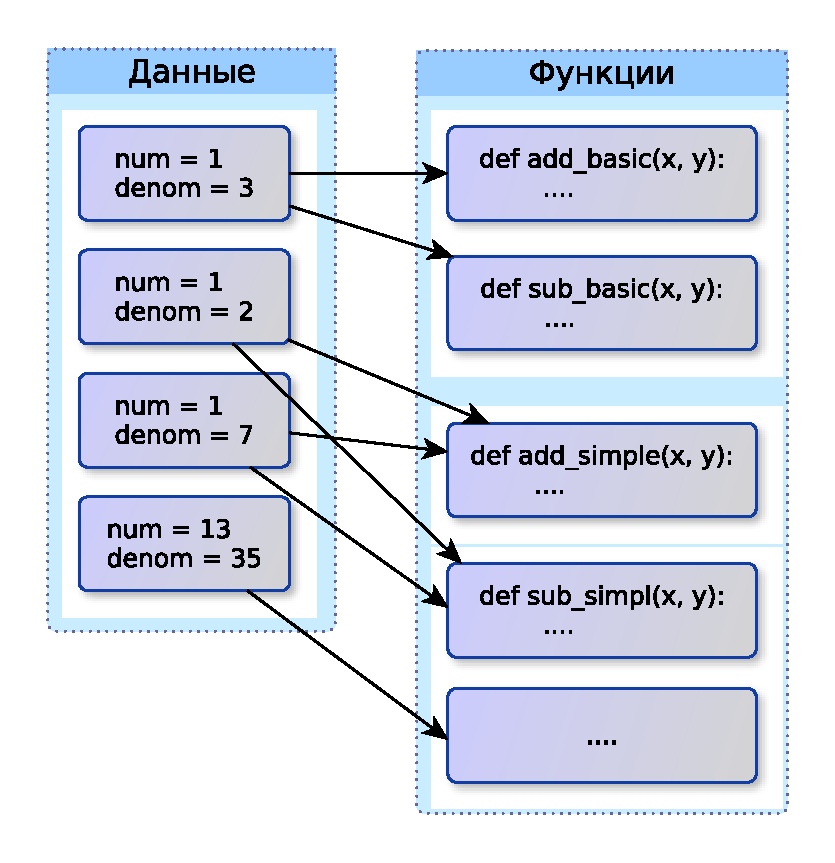
\includegraphics{images/semi_OOP_style.eps} \end{center} 
\newpage

%-------------------------------------------------------------------------------
\begin{center} Не совсем процедурный стиль - анализ \end{center}
\begin{itemize}
    \item Кода стало больше
    \item Его расширение упростилось - не нужно модифицировать функцию add,
          при добавлении нового типа
    \item Типовые теги стали менее нужны - тип это операции, которые есть у него
    \item Вместо \lstinline!func(x)! теперь \lstinline!x['func'](x)!. 
          Для упрощения вызова старая процедурная семантика оставлена,
          но внутри нее перенаправление на новый вызов
\end{itemize}
\newpage

%-------------------------------------------------------------------------------
\begin{center} Не совсем процедурный стиль - анализ \end{center}
\begin{itemize}
    \item Реализовывать новый метод для всех классов сложнее - нужно менять 
          код во многих местах.
    \item Типовые теги иногда нужны.
    \item Каждый экземпляр содержит большое количество ссылок на одни и те же
          функции.
    \item Решение - вынесение всех методов в отдельный словарь, который все 
          переменные данного типа используют совместно. Одновременно этот
          словарь становится типовым тегом.
\end{itemize}
\newpage

%-------------------------------------------------------------------------------
\begin{center} Рациональные числа - совсем не процедурный стиль \end{center}
\begin{lstlisting}
    BasicRN = {'add': add_basic, 
               'sub': sub_basic,
               '__init__': mk_basic}

    ASRN = {'add': add_simplified, 
            'sub': sub_simplified,
            '__init__': mk_simple}

    def new(tp):
        def closure(*args, **kwargs):
            return tp['__init__'](*args, **kwargs)
        return closure

    x1 = new(BasicRN)(1, 2)
    x2 = new(ASRN)(1, 2)

    def add(x, y):
        return x['__class__']['add'](x, y)
\end{lstlisting}
\newpage

%-------------------------------------------------------------------------------
\begin{center} Рациональные числа - совсем не процедурный стиль \end{center}
\begin{itemize}
    \item Шаблон, использованный в функции add часто используется в 
          python и позволяет имитировать перегрузку функций
    \item Почти так устроено ООП в питоне внутри
\end{itemize}
\newpage

%-------------------------------------------------------------------------------
\begin{center} 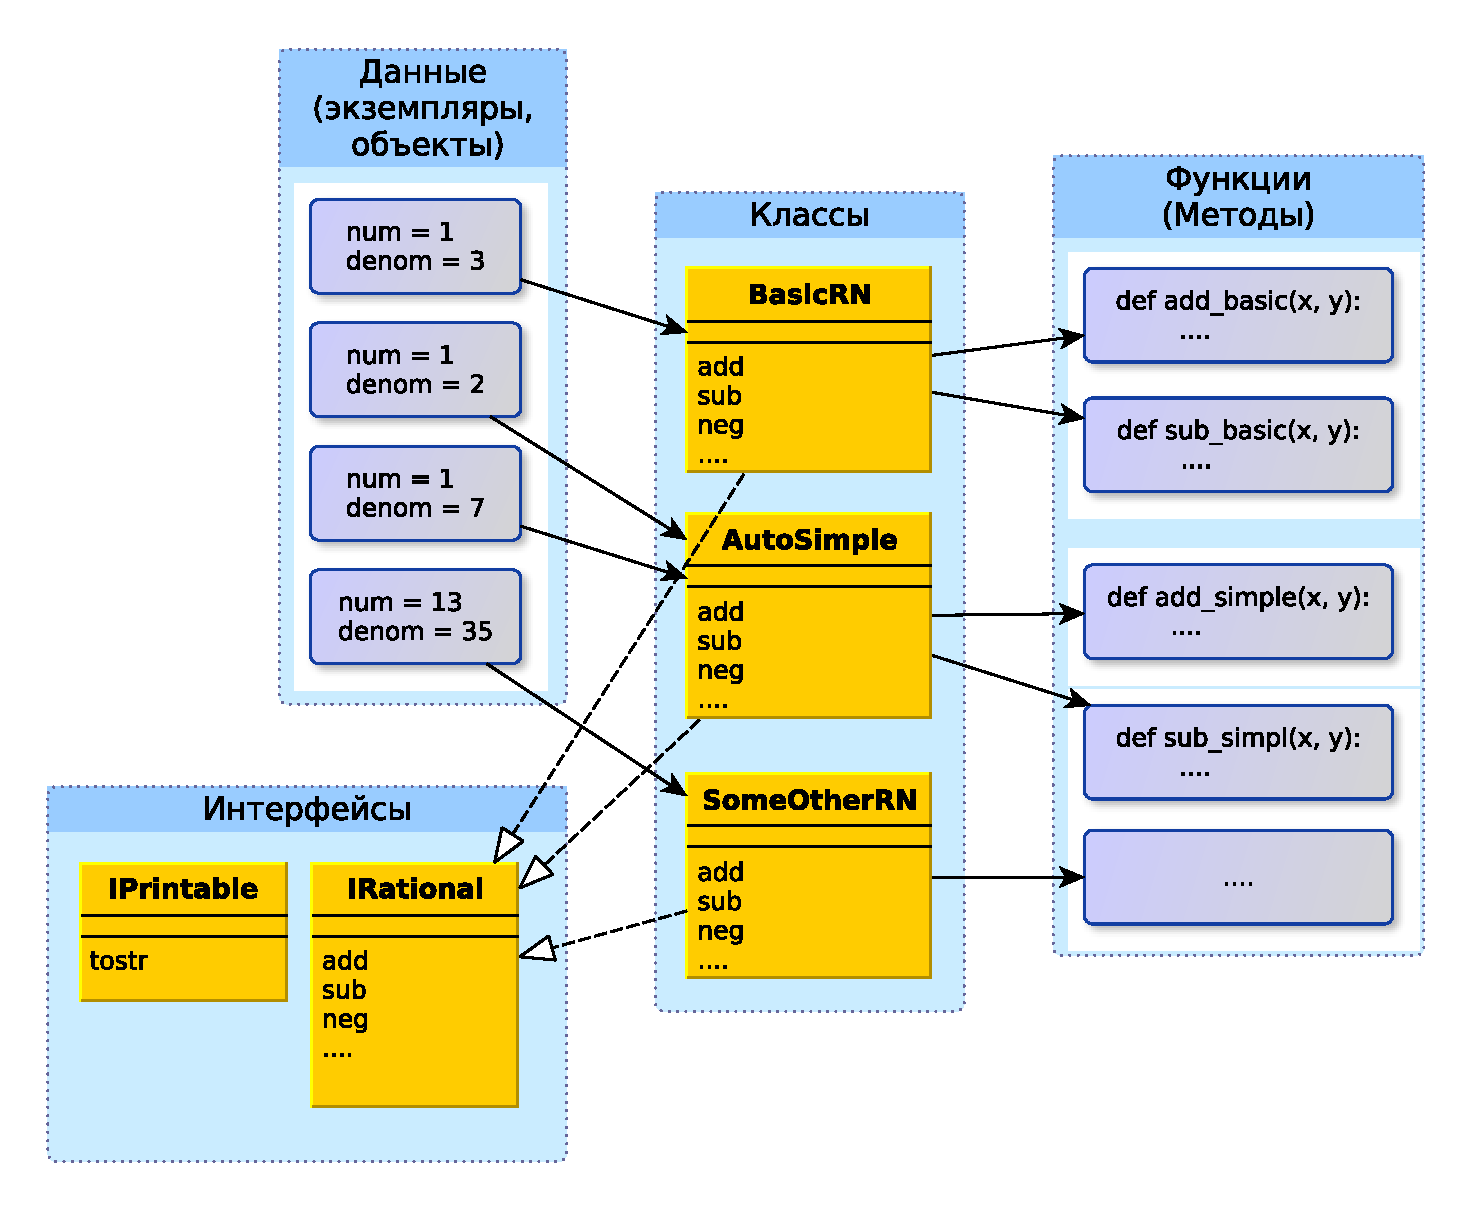
\includegraphics[scale=0.8]{images/oop_style.eps} \end{center} 
\newpage

%-------------------------------------------------------------------------------
\begin{center} 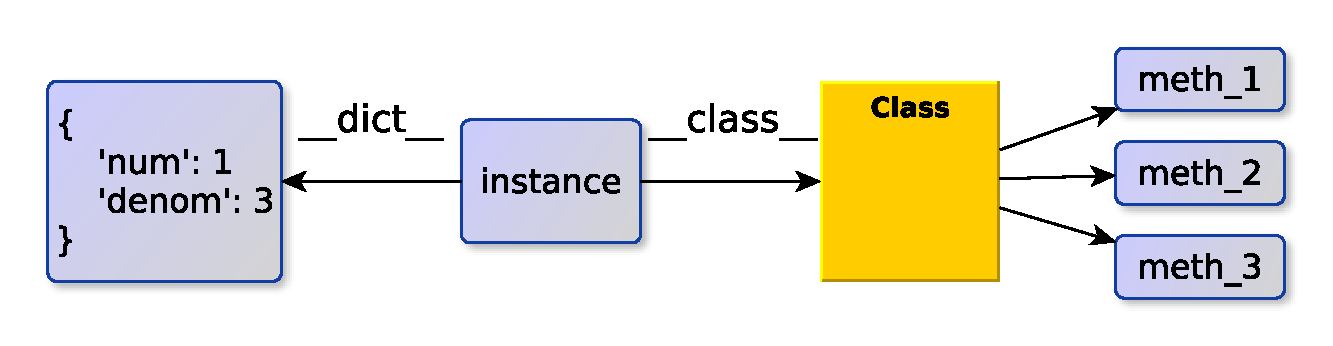
\includegraphics[scale=0.8]{images/python_instance.eps} \end{center} 
\lstinline!obj.__class__ == type(obj)! - класс объекта \\
\lstinline!obj.__dict__! - словарь, содержащий атрибуты объекта
\newpage

%-------------------------------------------------------------------------------
\begin{center} Рациональные числа - классы \end{center}
\begin{lstlisting}
    class BasicRational(object):
        "basic rational number"

        def __init__(self, num, denom):
            self.num = num
            self.denom = denom

        def add(self, y):
            nd = self.denom * y.denom
            nn = self.num * y.denom + y.num * self.denom
            return BasicRational(nn, nd)

        def neg(self):
            return BasicRational(-self.num, self.denom)

        def sub(self, y):
            return self.add(y.neg())

        def tostr(self):
            return "{0.num}/{0.denom}".format(self)
\end{lstlisting}
\newpage

%-------------------------------------------------------------------------------
\begin{center} Рациональные числа - классы \end{center}
\begin{lstlisting}
    class AutoSimpl(BasicRational):
        "Auto simplified rational number"

        def add(self, y):
            res = BasicRational.add(self, y)
            cur_gcd = gcd(res.num, res.denom)
            res.num /= cur_gcd
            res.denom /= cur_gcd
            return res
\end{lstlisting}
\newpage

%-------------------------------------------------------------------------------
\begin{center} Рациональные числа - классы \end{center}
\begin{lstlisting}
    class AutoSimpl(BasicRational):
        "Auto simplified rational number"
    
        def __init__(self, num, denom):
            cur_gcd = gcd(num, denom)
            self.num = num / cur_gcd
            self.denom = denom / cur_gcd
\end{lstlisting}
\newpage

%-------------------------------------------------------------------------------
\begin{center} ООП \end{center}
\begin{itemize}
    \item Шаблон проектирования, в котором данные имеют ссылки на функции их обработки
    \item Шаблон проектирования, в котором объекты обмениваются сообщениями, возможно,
          меняя при этом свое состояние
    \item Позволяет писать код, который сохраняет работоспособность при изменении данных
\end{itemize}
\newpage

%-------------------------------------------------------------------------------
\begin{center} ООП vs Процедурный стиль \end{center}
\begin{itemize}
    \item (-) Часто больше кода
    \item (-) Усложняет язык
    \item (-) Разработка ООП дизайна требует больших навыков, чем процедурного
    \item (-) Добавление нового метода требует нелокальных изменений
    \item (-) Работает только если функция выбирается по типу одного из параметров
    \item (+) Уменьшает пересечение имен
    \item (+) Код лучше структурирован
    \item (+) Избавляет от ручной проверки типов
    \item (+) В некоторых случаях значительно упрощается расширение
    \item (+) Позволяет корректно написанному коду работать с ноывми типами данных
    \item (+) Более высокий уровень абстракции упрощает построение программы
              путем выделения стандартных шаблонов проектирования
    \item (+) Многие из идей ООП имеют прямую поддержку в языке
\end{itemize}
\newpage

%-------------------------------------------------------------------------------
\begin{center} Python ООП vs Процедурный стиль \end{center}
\begin{itemize}
    \item Возможность перегрузки функций
    \item Возможность перегрузки операторов
    \item x.y => x.\_\_dict\_\_['y']
    \item x.func(...) => x.\_\_class\_\_.func(x, ...)
    \item x + y => x.\_\_add\_\_(y)
    \item -x => x.\_\_neg\_\_()
\end{itemize}
\newpage

%-------------------------------------------------------------------------------
\begin{center} Добавление метода ко всем классам сразу требует нелокальных изменений \end{center}
Один из вариантов решения - совместить стили.
\begin{lstlisting}
    def some_new_method(obj):
        if isinstance(obj, ClS1):
            # code for CLS1
        elif isinstance(obj, ClS2):
            # code for CLS2
        else:
            return obj.some_new_method()
\end{lstlisting}
\newpage

%-------------------------------------------------------------------------------
\begin{center} Рациональные числа - python way \end{center}
\begin{lstlisting}
    class BasicRational(object):
        "basic rational number"

        def __init__(self, num, denom):
            self.num = num
            self.denom = denom

        def __add__(self, y):
            nd = x.denom * y.denom
            nn = x.num * y.denom + x.denom * y.num
            return self.__class__(nn, nd)

        def __neg__(self):
            return self.__class__(-nn, nd)

        def __sub__(self, y):
            return self.add(y.neg())

        def __str__(self):
            return "{0.num}/{0.denom}".format(self)

        def __repr__(self):
            return str(self)

    b1 = AutoSimpl(1, 2)
    b2 = AutoSimpl(1, 3)
    b3 = b2 - b1 - b1
    print b1, b2, b3
\end{lstlisting}
\newpage

%-------------------------------------------------------------------------------
\end{document}
